\documentclass{article}
\usepackage{amsfonts}
\usepackage{amsmath}
\usepackage[UTF8]{ctex}
\usepackage{amsthm}
\usepackage{amssymb}
\usepackage{tikz}
\usepackage{multido}

\usetikzlibrary{decorations.markings}
\usetikzlibrary{shapes.geometric}
\usetikzlibrary{arrows}

\tikzstyle{startstop} = [rectangle,rounded corners,minimum width=3cm,minimum height=1cm,text centered,draw=black]
\tikzstyle{io} = [trapezium, trapezium left angle=70, trapezium right angle=110, minimum width=3cm, minimum height=1cm, text centered, draw=black]
\tikzstyle{process} = [rectangle, minimum width=3cm, minimum height=1cm, text centered, draw=black]
\tikzstyle{decision} = [diamond, minimum width=3cm, minimum height=1cm, text centered, draw=black]

\newenvironment{solution}{\renewcommand\qedsymbol{$\blacksquare$}\begin{proof}[解]}{\end{proof}}
\newenvironment{annotation}{\renewcommand\qedsymbol{}\begin{proof}[注]}{\end{proof}}

\newcommand{\nstars}[1]{\multido{}{#1}{$\star$}}

\title{RDCSS 2020:Newton力学小测验解答}
\author{詹有丘}

\begin{document}

\maketitle

\paragraph{问题1}\nstars{4}

\begin{solution}

将$t$写成矩阵的形式
$$t\left(a\right)=M^{\mathrm T}a,$$
其中
$$M:=\left[\begin{matrix}0\\1\\2\\-3\end{matrix}\right].$$
随意构造以$M$为法向的超平面(即$\operatorname{Ker}t$)的一组正交基,例如
$$\left[\begin{matrix}0\\0\\3\\2\end{matrix}\right],
\left[\begin{matrix}0\\13\\-2\\3\end{matrix}\right],
\left[\begin{matrix}1\\0\\0\\0\end{matrix}\right]$$
(不唯一).

将它们分别归一化,并拼成一个矩阵,得到
$$R:=\left[\begin{matrix}0&0&1\\0&\frac{13}{\sqrt{182}}&0\\\frac3{\sqrt{13}}&-\frac2{\sqrt{182}}&0\\\frac2{\sqrt{13}}&\frac3{\sqrt{182}}&0\end{matrix}\right].$$

然后双射$\varphi:a\mapsto Qa$即为所求同构,其中
$$Q:=\left[\begin{matrix}M^{\mathrm T}\\R^{\mathrm T}\end{matrix}\right]=\left[\begin{matrix}0&1&2&-3\\0&0&\frac3{\sqrt{13}}&\frac2{\sqrt{13}}\\0&\frac{13}{\sqrt{182}}&-\frac2{\sqrt{182}}&\frac3{\sqrt{182}}\\1&0&0&0\end{matrix}\right].$$

\end{solution}

\begin{annotation}
此题答案不唯一.
\end{annotation}

\paragraph{问题2}\nstars{4}

\begin{solution}

由题意写出势场
$$U=\frac12\left(l-l_0\right)^2=\frac12\left(\sqrt{x^2+d^2}-l_0\right)^2.$$

求导两次,得到
$$U'=x\left(1-\frac{l_0}{\sqrt{x^2+d^2}}\right),$$
$$U''=1-\frac{l_0}{\sqrt{x^2+d^2}}+\frac{l_0x^2}{\left(x^2+d^2\right)^\frac32}.$$

情形1:有$d>l_0$.

此时$U'$具有唯一零点$x=0$.

由于$U''\left(0\right)=1-l_0/d>0$,故$x=0$是稳定平衡位置,会出现微振动.其周期
$$T=\frac{2\pi}{\sqrt{U''\left(0\right)}}=2\pi\sqrt{\frac d{d-l_0}}.$$

情形2:有$d<l_0$.

此时$U'$具有三个零点$x=0,\pm\sqrt{l_0^2-d^2}$.

由于$U''\left(0\right)=1-l_0/d<0$,故$x=0$不是稳定平衡位置,不会出现微振动.

由于$U''\left(\pm\sqrt{l_0^2-d^2}\right)=1-d^2/l_0^2>0$,故$x=\pm\sqrt{l_0^2-d^2}$是稳定平衡位置,会出现微振动.其周期
$$T=\frac{2\pi}{\sqrt{U''\left(\pm\sqrt{l_0^2-d^2}\right)}}=
2\pi\sqrt{\frac{l_0^2}{l_0^2-d^2}}.$$

\end{solution}

\paragraph{问题3.1}\nstars{1}

\begin{solution}

$$T=\frac{\mathrm dS}{\mathrm dE}=2E.$$

\end{solution}

\paragraph{问题3.2}\nstars{3}

\begin{solution}

我们有
$$x=\pm\frac1{2\sqrt2\pi}\int_0^U\frac T{\sqrt{U-E}}\mathrm dE.$$
将第1问的结论代入上式,得到
$$x=\pm\frac1{\sqrt2\pi}\int_0^U\frac E{\sqrt{U-E}}\mathrm dE.$$

利用所提示的积分公式,可以算得
$$x=\pm\frac{2\sqrt2}{3\pi}U^\frac32,$$
即
$$U=kx^\frac23,$$
其中$k:=\sqrt[3]{9\pi^2}/2$.

\end{solution}

\begin{annotation}

有结论:势场$U=A\left|x\right|^n$中质点运动的周期为
$$T=\frac{2\sqrt{2\pi}\Gamma\left(\frac1n\right)}{nA^{\frac1n}\Gamma\left(\frac1n+\frac12\right)}E^{\frac1n-\frac12}.$$

\end{annotation}

\begin{annotation}

此题中,不具体计算就可以得到$U\propto x^\frac23$.方法:设$U\propto\left|x\right|^n$,则根据力学相似性,当线度变化$\alpha$倍时,能量变化$\alpha^n$倍,而时间变化$\alpha^{1-n/2}$倍.由$T\propto E$可知$n=1-n/2$,故有$n=2/3$.

\end{annotation}

\paragraph{问题4.1}\nstars{3}

\begin{proof}

用数学归纳法.

首先,当$\omega=0$时原命题显然.当$\omega=1$时原命题显然.

假设当$\omega=k-1$时和当$\omega=k$时原命题都成立.

考虑到
$$\cos\left(\left(k+1\right)x\right)=\cos\left(kx\right)\cos x-\sin\left(kx\right)\sin x$$
且
$$\cos\left(\left(k-1\right)x\right)=\cos\left(kx\right)\cos x+\sin\left(kx\right)\sin x,$$
将两式相加,得
$$\cos\left(\left(k+1\right)x\right)+\cos\left(\left(k-1\right)x\right)=2\cos\left(kx\right).$$

由此结合归纳假设,容易得到当$\omega=k+1$时,原命题成立.

\end{proof}

\begin{proof}

由De Moivre公式,有
$$\cos\omega x+\mathrm i\sin\omega x=\left(\cos x+\mathrm i\sin x\right)^\omega.$$
将上式右边用Newton二项式定理展开,得
$$\cos\omega x+\mathrm i\sin\omega x=\sum_{k=0}^\omega\binom\omega k\left(\cos x\right)^{\omega-k}\left(\mathrm i\sin x\right)^{2k}.$$
将上式两边同时取实部.当$k$为偶数时,被求和式为实数.故有
$$\cos\omega x=\sum_{k=0}^{\left\lfloor\frac\omega2\right\rfloor}\binom\omega{2k}\left(\cos x\right)^{\omega-2k}\left(-1\right)^k\left(\sin x\right)^{2k}.$$
由$\left(\sin x\right)^2=1-\left(\cos x\right)^2$得
$$\cos\omega x=\sum_{k=0}^{\left\lfloor\frac\omega2\right\rfloor}\binom\omega{2k}\left(\cos x\right)^{\omega-2k}\left(\left(\cos x\right)^2-1\right)^k.$$

于是$\cos\omega x$被表示为$\left\lfloor\omega/2\right\rfloor$个关于$\cos x$的$\omega$次多项式之和.由此得知原命题成立.

\end{proof}

\paragraph{问题4.2}\nstars{2}

\begin{solution}

考虑到递推关系
$$f\left(2^{k+1},x\right)=2f\left(2^k,x\right)^2-1$$
后发现,只需$n$次循环即可计算出$f\left(2^n,x\right)$.

使用如下Python代码:
\begin{verbatim}
r = float(input())
for k in range(int(input())):
    r = 2*r*r - 1
print(r)
\end{verbatim}

或者如下流程图:

\begin{tikzpicture}[node distance=2cm]
\node (start) [startstop] {开始};
\node (in) [io, below of=start, yshift=0.5cm] {输入$r$(即$\cos x$)和$n$};
\node (init) [process, below of=in, yshift=0.5cm] {$k\leftarrow0$};
\node (while) [decision, below of=init] {$k<n$?};
\node (cyc) [process, below of=while, yshift=-0.5cm] {$\begin{matrix}r\leftarrow 2r^2-1\\k\leftarrow k+1\end{matrix}$};
\node (out) [io, right of=while, xshift=2cm] {输出$r$};
\node (stop) [startstop, below of=cyc] {结束};

\draw [->] (start) -- (in);
\draw [->] (in) -- (init);
\draw [->] (init) -- (while);
\draw [->] (while) -- node[anchor=west] {是} (cyc);
\draw [->] (while) -- node[anchor=north] {否} (out);
\draw [->] (cyc) -- ++(-3cm,0) |- ++(3cm,3.7cm);
\draw [->] (out) |- (stop);
\end{tikzpicture}

\end{solution}

\begin{annotation}

此算法在实际使用中存在很大的精度问题.

\end{annotation}

\paragraph{问题5.1}\nstars{1}

\begin{solution}

先作出$U$-$x$图,
然后在$U$-$x$图上画一些能级.
如下图所示.

\begin{tikzpicture}
\draw[->] (-3.5,0) -- (3.5,0) node[anchor=north] {$x$};
\draw[->] (0,-0.5) -- (0,2) node[anchor=west] {$U$};
\draw[domain=0:3.5,variable=\x] plot ({\x},{\x^2/8});
\draw[domain=-3.5:0,variable=\x] plot ({\x},{-\x^2/8});
\draw[dashed] (-1,0.125) -- (1,0.125);
\draw[dashed] (-2,0.5) -- (2,0.5);
\draw[dashed] (-3,1.125) -- (3,1.125);
\end{tikzpicture}

在相图中画出能级对应的等能集,
再标上箭头即得相曲线.

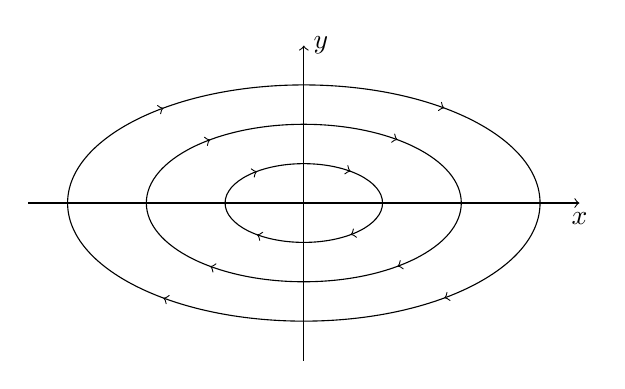
\begin{tikzpicture}
\draw[->] (-3.5,0) -- (3.5,0) node[anchor=north] {$x$};
\draw[->] (0,-2) -- (0,2) node[anchor=west] {$y$};
\begin{scope}[decoration={markings,
	mark=at position 0.125 with {\arrowreversed{>}},
	mark=at position 0.375 with {\arrowreversed{>}},
	mark=at position 0.625 with {\arrowreversed{>}},
	mark=at position 0.875 with {\arrowreversed{>}}}]
\draw[postaction={decorate}] (0,0) ellipse (1 and 0.5);
\draw[postaction={decorate}] (0,0) ellipse (2 and 1);
\draw[postaction={decorate}] (0,0) ellipse (3 and 1.5);
\end{scope}
\end{tikzpicture}

所求的相曲线如上图所示.

\end{solution}

\begin{proof}

能量$E$对应的相曲线为曲线$y^2/2+kx^2=E$,为半轴长分别为$\sqrt{E/k}$和$\sqrt{2E}$的椭圆.

\end{proof}

\paragraph{问题5.2}\nstars{2}

\begin{proof}

运动方程为
$$\ddot x_1=-2kx_1,\quad\ddot x_2=-2kx_2.$$

容易解得
$$\mathbf x=\mathbf A\left[\begin{matrix}\cos2kt\\\sin2kt\end{matrix}\right],$$
其中$\mathbf x:=\left[\begin{matrix}x_1\\x_2\end{matrix}\right]$,且$\mathbf A\in\mathbb R^{2\times2}$.
两边左乘$\mathbf A^{-1}$,得
$$\mathbf A^{-1}\mathbf x=\left[\begin{matrix}\cos2kt\\\sin2kt\end{matrix}\right].$$
两边左乘自身的转置,利用正余弦平方和为$1$,得
$$\mathbf x^{\mathrm T}\left(\mathbf A^{-1}\right)^\mathrm T\mathbf A^{-1}\mathbf x=1.$$
因此轨迹是系数为$\mathbf M:=\left(\mathbf A^{-1}\right)^\mathrm T\mathbf A^{-1}$的二次曲线.

因为$\left|\mathbf M\right|=\left|\mathbf A^{-1}\right|^2>0$,故轨迹是椭圆.

特殊地,若$\mathbf A^{-1}$不存在,则轨迹退化为线段或点.

\end{proof}

\paragraph{问题5.3}\nstars{1}

\begin{proof}

在有心力场中角动量守恒.由于角动量与位置和速度都垂直,故位置和速度只能在以角动量为法向量的平面内变化.运动退化为二维的.

由第2问可知,二维情形中轨迹为椭圆.故三维情形中轨迹也为椭圆.

特殊地,若角动量为零,则轨迹退化为线段或点.

\end{proof}

\paragraph{问题5.4}\nstars{3}

\begin{proof}

设初速度与初位置张成的二维平面为$V$,
且$V$在$\mathbb R^4$中的正交补为$V^\perp$.

设$\mathbf A$为以$V$中的一组标准正交基为列向量的$4\times2$矩阵,
而$\mathbf B$为以$V^\perp$中的一组标准正交基为列向量的$4\times2$矩阵,
再令$4\times4$矩阵$\mathbf Q:=\left[\begin{matrix}\mathbf A&\mathbf B\end{matrix}\right]$,则
$$\mathbf R:=\mathbf Q\left[\begin{matrix}1\\&1\\&&-1\\&&&-1\end{matrix}\right]\mathbf Q^\mathrm T$$
为正交矩阵,且$\mathbf v=\mathbf R\mathbf v$当且仅当$\mathbf v\in V$.

由于势场和初条件在$\mathbf R$对应的正交变换下不变,
故该系统的运动也在该正交变换下不变,
即运动始终停留在平面$V$上,运动退化为二维的.

由第2问可知,二维情形中轨迹为椭圆.故四维情形中轨迹也为椭圆.

特殊地,若初速度和初位置线性相关(即无法张成二维平面$V$),则轨迹退化为线段或点.

\end{proof}

\paragraph{问题6}\nstars{5}

\begin{proof}

在二体问题中,质心为
$$\mathbf r_0=\frac{m_1\mathbf r_1+m_2\mathbf r_2}{m_1+m_2}.$$
故当$m_1\to\infty$时,
有$\mathbf r_0=\mathbf r_1$,
故$\mathbf v_0=\mathbf v_1$.

另一方面,由于动量守恒,有$\mathbf v_0=\mathrm{const}$.
故在$m_1\to\infty$时有$\mathbf v_1=\mathrm{const}$.
因此在$m_1$初始静止的参考系中$m_1$将始终静止.

在二体问题中,相对位置$\mathbf r:=\mathbf r_2-\mathbf r_1$的变化,
如同具有质量$$m:=\frac{m_1m_2}{m_1+m_2}$$的质点在场$U\left(r\right)$中的运动.
即,如同单位质量的质点在场$W=U/m$中的运动.

注意到当$m_1\to\infty$时,有$m=m_2$,即有$W=V$.
因此$m_2$相对于$m_1$的运动相当于具有单位质量的质点在场$V$中的运动.

\end{proof}

\end{document}
